\documentclass[twocolumn]{article}
\usepackage{cite}
\usepackage{amsmath,amssymb,amsfonts}
\usepackage{algorithmic}
\usepackage{graphicx}
\usepackage{textcomp}
\usepackage{xcolor}
\usepackage{multicol}
\usepackage{float}

\def\BibTeX{{\rm B\kern-.05em{\sc i\kern-.025em b}\kern-.08em
    T\kern-.1667em\lower.7ex\hbox{E}\kern-.125emX}}
   \date{}
\begin{document}

\begin{titlepage}
    \begin{center}
        \vspace{1cm}
        \normalsize
        \textbf{Project Report on}\\
        \vspace{0.5cm}

        \Large
        \textbf{Human Activity Recognition from video sequences using Deep Learning}\\
        \vspace{0.5cm}
        \emph{Submitted by}\\
        \vspace{0.5cm}
        \large
        \textbf{Amit Kumar} \hspace{0.75cm}
        \textbf{B190343CS}\\
        \textbf{Uttkarsh Raj} \hspace{0.75cm}
        \textbf{B190955CS}\\
        \textbf{Moturu Manogna} \hspace{0.75cm}
        \textbf{B190695CS}\\
        %\textbf{Group Members:}\\
        %\vfill
        \vspace{0.2cm}
        \emph{Under the Guidance of}\\
        \large
        \vspace{0.5cm}
        \textbf{Pournami PN}

        \vspace{.5cm}
        \begin{center}
            
\includegraphics[width=0.4\textwidth]{nitc-logo.png}
        \end{center}
        \vspace{0.8cm}
        \textbf{Department of Computer Science and Engineering}\\
        \textbf{National Institute of Technology Calicut}\\
        \textbf{Calicut, Kerala, India - 673 601}\\
        \vspace{0.8cm}
        \textbf{November 15, 2022} %Enter the date
    \end{center}
\end{titlepage}

\title{\textbf{Human Activity Recognition from video sequences using Deep Learning}}\\
\author{Amit Kumar \and Uttkarsh Raj \and Moturu Manogna}

\twocolumn[
    \begin{@twocolumnfalse}
        \maketitle
        \textbf{
            \textit\textbf{{Abstract:}}
            AI is replacing humans in various laborious tasks, including watching video
            surveillance streams to detect unusual actions at airports, railway stations, bus stops, and other
            public gatherings, summarising human actions in a video, etc. A human doing these activities
            leaves a scope of error due to negligence and is cost-ineffective. Our project is to identify human activities
            and the time in the video at which that activity took place using deep learning and video data processing methods.
            Unlike image processing, video processing requires many input parameters and computational power to train the
            model. Our model takes a video clip as input and outputs the name of the activity in the video.
        }\vspace{0.5cm}
    \end{@twocolumnfalse}
]


\section{Introduction}
Human activity recognition is the task of identifying activities done by a human in a live video stream, recorded video clip, or sequence of images. For example, walking,
Running, dancing, playing cricket, jumping, etc. The two goals involved in a HAR system are to identify the activity and the time of activity in video. This data is
further used to trigger some actions. HAR systems can be used along with video surveillance cameras to enhance security and well-being by identifying suspicious
activities, crimes, and accidents in public places like airports, bus stands, forests, mountains, and other remote areas. There are many applications of the HAR
system in healthcare, like monitoring patient activities, developing human-computer interfaces like giving commands to computers through hand actions, virtual reality,
and military uses like identifying terrorist activities, etc. An alert is generated in HAR systems on certain human activities, which is further sent to the control room
for further inspection or trigger some actions. HAR systems reduce the scope of error due to human negligence in surveillance systems, reduce the cost of monitoring
and deployment, and can be easily deployed to cover large and remote areas. \\
Types of HAR Systems:
On the basis of equipment, there are two main categories of HAR (Human Activity Recognition) systems :
Vision-Based Human Activity Recognition and Sensor-Based Human Activity Recognition.\\
Vision-Based Human Activity Recognition:
Vision-Based HAR is the task of capturing the video by installing static cameras at various places for observation purposes and sending it to the servers.
These camera security footages or camera-recorded clips are used to keep an eye and predict the movement of humans using that recording. We can use this type of HAR for
security, the medical field, visual monitoring, irregular behavior detection, road safety, crowd monitoring, etc. In vision-based HAR, only camera recordings are used, no
sensors are used for action recognition.\\
Sensor-Based Human Activity Recognition:
Sensor-Based HAR is a technology that can recognize human activities through sensors. In this method, data is fetched from the sensors, which can either be present in
smartphones or any wearable device. In vision-based HAR, cameras are installed at fixed positions, so action recognition is limited. In sensor-based HAR, data received
from sensors is for a specific task, but in the case of cameras, it contains data
from another non-target human in the view angle. For sensors, there is no limitation on the position of sensors.

\section{Problem statement}
To design and develop a vision-based human activity recognition system to identify human activities and the time of the activity in a video. The input to this system will be a video clip. The output will be the name of the activity in the video.

\section{Literature Review}
\cite{b1} This paper discusses video processing using deep learning techniques. It discusses the applications of video processing in real life like entertainment, surveillance, crowd
management etc, functionalities of video processing in computer vision context like Human Action Recognition (HAR), motion detection, object detection, object recognition, object tracking,
video classification, behavior analysis, background subtraction, event recognition, action segmentation and scene understanding. The paper further talks about the techniques used for video processing,
data sets generally used to train the model and the challenges faced like poor quality of videos, complexity in tracking and locating multisubject, dynamic backgrounds, and lack of open research
datasets and computation power.\\

\cite{b2} This paper discusses the problems faced in Human Activity Recognition and the research which have been done on video processing.
A review of different types of video-based HAR methods, i) HandCrafted Feature-Based Approach, ii) Deep Learning Approach, and various benchmark video datasets are given.
Deep learning methods like CNN (Convolutional Neural Network) approach, RNN (Recurrent Neural Network), and LSTM (Long Short Term Memory) with CNN are reviewed with all the details
about the study done on these topics. The paper expresses low-quality videos, lack of dataset, complex and dynamic background and activities, and design constraints of real-time HAR video systems
as major challenges.\\

\cite{b3} This paper discusses deep learning techniques used for video-based human action recognition. The paper discusses current state-of-the-art human action recognition
systems built using Convolution Neural Networks (CNNs), Recurrent Neural Networks - Long Short Term Memory (RNN-LSTMs), Deep Belief Networks (DBNs), and Stacked Denoising Autoencoders(SDAs).
The paper also discusses the future research directions in the field of human action recognition, like developing unsupervised learning models, as the cost of labeling data is very high
in terms of money and manpower, developing deeper CNNs, combining different learning models in a single framework, fusion of hand-crafted and deep learning solutions, and using transfer learning.\\

\cite{b4} This paper discusses various video-based Human Activity Detection(HAD) approaches. The paper discusses various state-of-the-art HAD approaches based on the number of actors/objects- Single-person activity, and multiple person activity which are further classified and analyzed in detail. An analysis of Deep-learning based HAD techniques like CNN, DB-LSTM, 3D CNN, and 2D CNN is done. The CNN on datasets USCD Ped1, USCD Ped2, CUHK with 98.5\% accuracy is the most accurate. They further compared various benchmark datasets including UCF101, MSR-1, UFC sports, KTH. The paper expresses multiple actions detection, multiview-invariance and occlusion,
interclass similarity and intra-class variation as major challenges.\\

% \cite{b14} This paper provides analysis on HAR using CNN and LSTM. They provided a detailed explanation on CNN, LSTM, Hybrid model of CNN and LSTM. They performed EDA on dataset WISDM, implemented CNN and LSTM models on the dataset WISDM and compared the results. The results showed that the CNN model has far better accuracy terms compared with the LSTM model with an accuracy of 99.593\%. 

\subsection{Vision-based HAR Methods}
Researchers have presented many handcrafted feature-based and deep learning-based approaches over the decade. However, deep learning-based HAR techniques are used over
the handcrafted-feature-based approach because in the latter, the commonly used extractors are developed based on a specific dataset, and the extractors are database-biased, general
purpose feature extraction ability is absent, and it is a labor-intensive and time-consuming technique.

\subsubsection{CNN based}
CNNs are one of the most popular neural deep learning models used to process visual data and are used for image processing. One significant benefit of CNNs is that they can operate directly on raw data without requiring any hand-crafted feature extraction. A video can be divided into a sequence of images, and CNN can be applied to each of the images.\\
\cite{b5} The two-stream convolutional network proposed by Sismonyan and Zisserman has shown strong performance for human action recognition in videos. This model is a two-stream architecture including the spatial stream and the temporal stream, where each stream is executed by a
CNN. The first stream recognizes actions from a single frame, while the second recognizes actions from motion information of multi-frame optical flow. These two streams are then combined for the classification task. It showed a very good performance with limited training data. However, the two-stream architecture is not applicable for human
activity recognition in live video cameras due to higher computational complexity.\\
\cite{b6} The paper proposes a real-time human activity recognition using only Resnet and 3D CNN. The 2D Resnet-18 is converted to 3D CNN to capture spatial and time-related features from raw input. The network's rate of learning is fixed as $10^{−-3}$. The neural network uses 16 frame clips at the time of training. The Kinetics 400 dataset is used to train the model to avoid overfitting.

\subsubsection{CNN + LSTM based}
Video classification is more than just a simple image classification. To model complex dynamics of different actions, a Recurrent Neural Network (RNN) with long short-term memory(LSTM) is used because RNN allows us to access the long-range information of a temporal sequence.\\
\cite{b7} The authors proposed a novel technique that combines CNN and deep bidirectional LSTM network(DB-LSTM). Deep features are extracted from every sixth frame of the videos. Then, sequential information is learned from the frames using DB-LSTM. This model is capable of learning long-term sequences and can process lengthy videos by analyzing features for a certain time interval.\\
\cite{b8} Another approach using CNN and LSTM/BiLSTM is proposed in this paper. 90 frames after equal intervals are selected from the videos. Each frame of the video is converted to 299*299 dimensions and is sent to Inception-V3 and Xception CNN networks. Two models are built for training. In one the output of CNN networks is sent to the LSTM model and in another, to the BiLSTM model. Five activities from HMDB51 and UFC101 are selected for training. The models achieve test accuracy of 80.75\% using Inception -v3 and BiLSTM, 80.12\% using Inception-v3 and LSTM, and 77.02\% using Xception and LSTM.\\
\cite{b9} This paper purposed a novel hybridization deep learning model for comprehending and interpreting videos in HAR systems. They proposed a hybridization model to be built using 2D-Convolutional (2D-CNN) and stacked parallel bidirectional Long short-term memory. This model is capable of learning prolonged sequences and processing longer videos that are sequentially synchronized by accessing attributes over a specified time interval. They used two datasets UCF101 and SPHAR (Surveillance Perspective Human Action Recognition) for experiment and testing and to validate the proposed work.\\
\cite{b10} This paper used three different methods Two-stream CNN, CNN + LSTM, and 3D CNN. Every method is explicated and analyzed in detail. For training purposes HMDB-51 dataset. There are four actions to be classified in this paper namely clapping, waving, hugging, and drinking. All the methods give different accuracy when tested on the HMDB-51 dataset which contains 51 classes and 6766 short videos. The CNN + LSTM was the most accurate with an accuracy of 89.74\% followed by 3D CNN with an accuracy of 86.54\% and the least accuracy was Two-stream CNN with an accuracy of 82.37\%.\\

\subsection{Datasets}
Some of the benchmark HAR datasets that will be used to train and test the system are
\begin{itemize}
    \item \cite{b11} UFC101 dataset contains 132320 realistic action videos taken from youtube that are divided into 101 categories with 100-200 videos in each category.
    \item \cite{b12} HMDB51 dataset contains 6849 action video clips divided into 51 classes, each containing more than 100 clips.
\end{itemize}
\begin{figure}
    \center
    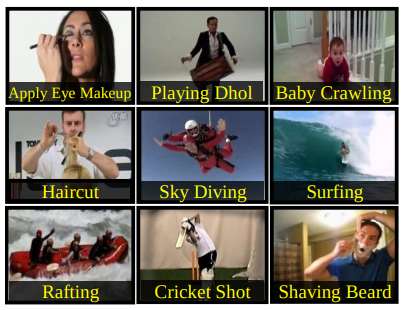
\includegraphics[width=0.4\textwidth]{UFC 101.png}
    \caption{Sample frames from classes in UFC101 \cite{b11}}
    \center
\end{figure}
\begin{figure}
    \center
    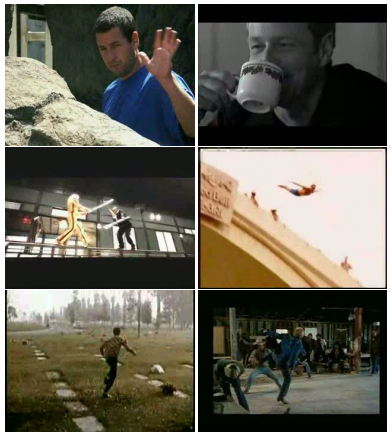
\includegraphics[width=0.4\textwidth]{HMDB51.png}
    \caption{Sample frames from classes in HMDB51 (from top-left to bottom-right hand-waving, drinking, sword fighting, diving, running and kicking)\cite{b12}}
    \center
\end{figure}

\section {Project Design}
As shown in figure 3, the video input is processed to get individual frames without affecting the sequence of action. The frames are then passed to ConvNet model which processes each frame. The output of this model is given to the LSTM model sequentially. In the end, the final state uses a softmax activation to get the label of the activity.
\begin{figure*}[h]
    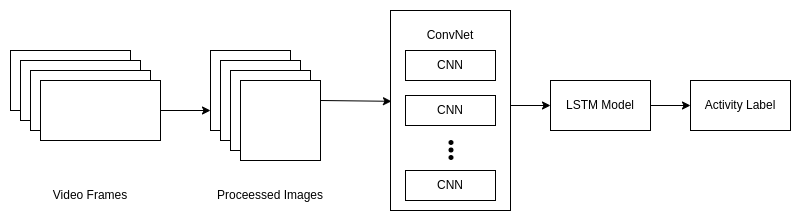
\includegraphics[width=\textwidth,height=4cm]{architecture.png}
    \caption{Design of the system}
\end{figure*}
\begin{figure}
    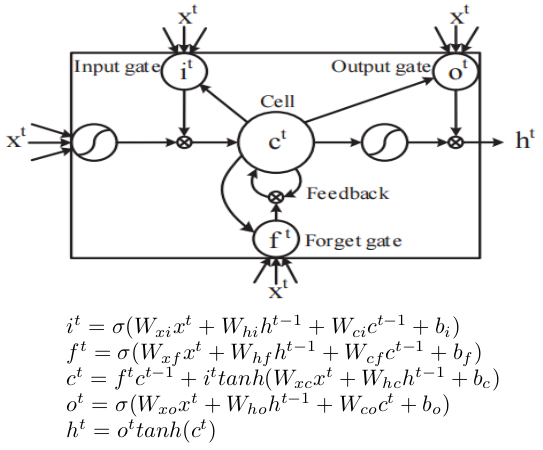
\includegraphics[width=0.5\textwidth]{LSTM Cell.png}
    \caption{Diagram of an LSTM unit (i is input gate, f is forget gate, o is output gate, h is output state and c is memory state) \cite{b3}}
\end{figure}
\begin{figure}
    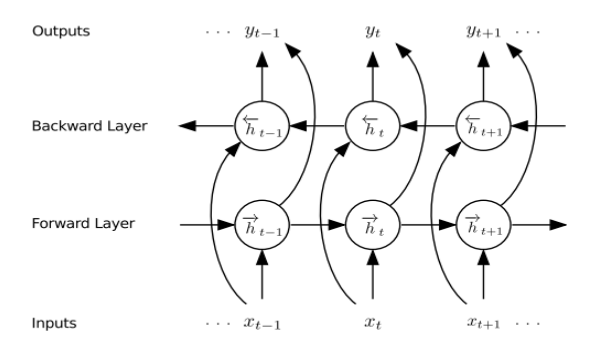
\includegraphics[width=0.5\textwidth,height=4cm]{BiLSTM.png}
    \caption{Architecture of a Bi-Directional LSTM \cite{b3}}
\end{figure}
\begin{figure}
    \center
    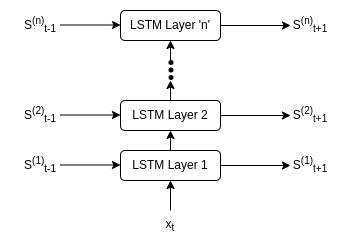
\includegraphics[width=0.4\textwidth,height=4cm]{Layered LSTM.drawio.png}
    \caption{N Layered LSTM}
    \center
\end{figure}
\subsection{Preprocessing}
This will include selecting frames from the video after certain jumps to avoid redundancies and to get an equal number of frames for all videos. The count of frames for each video will affect the size of the model, running time, and parameters of the ConvNet and LSTM models. After getting the frames, the frames will be resized to a square shape with the same dimensions for all the frames.

\subsection{ConvNet model}
A Convolutional neural network is used to extract spatial features from the video frames. The model will be run on each of the extracted video frames. The model architecture used is EfficientNet \cite{b13}. The base EfficientNet-B0 network is based on the inverted bottleneck residual blocks of MobileNetV2, in addition to squeeze-and-excitation blocks. EfficientNet uses a technique called compound coefficient to scale up models in a simple but effective manner. Instead of randomly scaling up width, depth or resolution, compound scaling uniformly scales each dimension with a certain fixed set of scaling coefficients. The EfficientNet outperforms all previous CNN architectures on most of the benchmark datasets and also transfers well.

\subsection{LSTM model}
LSTMs (figure 4) are used to extract temporal features from the sequence of video frames. They are used to overcome the gradient vanishing problem of traditional RNNs. Complex sequence patterns are not identified by the single LSTM Cell. Multiple LSTM cells are stacked together to learn long term dependencies in video data. To improve the performance, two LSTMs are stacked on top of each other, one in the forward direction and another in the backward direction to form a bi-directional LSTM (figure 5). The output is computed based on the hidden state of both LSTMs. Further, the performance is boosted by increasing the number of layers in this model as shown in figure 6. For example, layer 1 receives input from data while input of layer 2 is from its previous time steps and output of the current time step of layer 1. The output from the ConvNet model is given frame by frame to the LTSM model.

\section{Work Done}
\begin{itemize}
    \item Identified the problem domain, formulated the problem statement, and mentioned the input and output specifications.
    \item Gone through machine learning, convolutional neural networks courses on Coursera and recurrent neural networks, and read articles on the same.
    \item Done a thorough literature survey on commonly used techniques used in human activity recognition systems.
    \item Identified the datasets that will be used for training and testing the system.
    \item Created the base design of the system.
\end{itemize}

\section{Work Plan}
\begin{itemize}
    \item Go through video processing techniques and libraries for preprocessing the dataset.
    \item Go through PyTorch and other libraries to be used for implementing the model.
    \item Preprocessing the dataset to be used for training and testing the model.
    \item Implementing the model as per the design.
    \item Training and testing the implemented model.
\end{itemize}

\section{Conclusion}
We have successfully identified the problem domain, formulated the problem statement, and mentioned the input and output. We have studied various research papers in the field and learned some useful deep-learning techniques like CNNs, RNNs and LSTMs. We have finalized the datasets - UFC101 and HMDB51 to be used to train and test the system. We have created the base design of the system. Next, we will proceed with implementing, training and testing the system.


\begin{thebibliography}{00}
    \bibitem{b1}: Vijeta Sharma, Manjari Gupta, Ajai Kumari, and Deepti Mishra (2021) Video Processing Using Deep Learning Techniques: A Systematic Literature Review
    \bibitem{b2}: Vijeta Sharma, Manjari Gupta, Anil Kumar Pandey, Deepti Mishra, and Ajai Kumar (2022) A Review of Deep Learning-based Human Activity Recognition on Benchmark Video Datasets
    \bibitem{b3}: Hieu H. Pham, Louahdi Khoudour, Alain Crouzil, Pablo Zegers, and Sergio A. Velastin (2022) Video-based Human Action Recognition using Deep Learning: A Review
    \bibitem{b4}: I.Gull, Arvind. S and A. Sabha, "An Analysis of Video-based Human Activity Detection Approaches",2022 International Conference on Sustainable Computing and Data Communication Systems, 2022, DOI 10.1109/ICSCDS53736.2022.9760868.
    \bibitem{b5}: K. Simonyan and A. Zisserman, "Two-stream convolutional networks for action recognition in videos," in Advances in Neural Information Processing Systems, 2014
    \bibitem{b6}: N. Archana and K. Hareesh, "Real-time Human Activity Recognition Using ResNet and 3D Convolutional Neural Networks," 2021 2nd International Conference on Advances in Computing, Communication, Embedded and Secure Systems (ACCESS), 2021, pp. 173-177, doi: 10.1109/ACCESS51619.2021.9563316.
    \bibitem{b7}: A. Ullah, J. Ahmad, K. Muhammad, M. Sajjad and S. W. Baik, "Action Recognition in Video Sequences using Deep Bi-Directional LSTM With CNN Features," in IEEE Access, vol. 6, pp. 1155-1166, 2018, doi: 10.1109/ACCESS.2017.2778011.
    \bibitem{b8}: Vincent, Rajiv & Wagadre, Akshat & Sivaraman, Arun Kumar & M, Rajesh & Rajesh, Arun. (2020). Human Activity Recognition Using LSTM/BiLSTM. International Journal of Advanced Science and Technology. 7468-7474.
    \bibitem{b9}: A. Manaf F and S. Singh, "A Novel Hybridization Model for Human Activity Recognition using Stacked Parallel LSTMs with 2D-CNN for Feature Extraction," 2021 12th International Conference on Computing Communication and Networking Technologies (ICCCNT), 2021, pp. 1-7, doi: 10.1109/ICCCNT51525.2021.9579686.
    \bibitem{b10}: Z. Yu and W. Q. Yan, "Human Action Recognition Using Deep Learning Methods," 2020 35th International Conference on Image and Vision Computing New Zealand (IVCNZ), 2020, pp. 1-6, doi: 10.1109/IVCNZ51579.2020.9290594.

    \bibitem{b11}: Soomro, K., A. Roshan Zamir, and M. Shah. 2012. "UCF101: A Dataset of 101 Human Actions Classes From Videos in The Wild". November. http://arxiv.org/abs/1212.0402 .
    \bibitem{b12}: Kuehne, H., H. Jhuang, E. Garrote, T. Poggio, and T. Serre. 2011. HMDB: A Large Video Database for Human Motion Recognition, 2011 International Conference on Computer Vision, 2011, pp. 2556-2563, DOI: 10.1109/ICCV.2011.6126543
    \bibitem{b13}: Tan, M., & Le, Q. v. (2019). EfficientNet: Rethinking model scaling for convolutional neural networks. 36th International Conference on Machine Learning, ICML 2019, 2019-
    % \bibitem{b14}: Ch. Shiranthika, N. Premakumara, H. Samani, C.  Shyalika ,Huei-Ling Chiu, Chan-Yun Yang, "Human Activity Recognition Using CNN & LSTM" , 2020.

\end{thebibliography}


\end{document}
